\documentclass[a4,12pt]{scrartcl}

%Basic 
\usepackage[utf8]{inputenc}
\usepackage[ngerman]{babel}
\usepackage[T1]{fontenc}
\usepackage{float}
%\usepackage[bottom = 3.50cm]{geometry}

%Titel Seite
\title{CLOUD INFRASTRUCTURE}
\subtitle{Lab-04}
\author{Giorgio Vincenti und Samuel Krieg}
\date{\today}


%Kopf, Fusszeile
\usepackage{fancyhdr}
\pagestyle{fancy}
\lhead{ \begin{picture}(0,0) \put(0,0){
\includegraphics[width=3cm]{./pictures/hsrlogo.png}} \end{picture}}
\chead{}
\rhead{Seite \thepage}
\lfoot{Cloud Infrastructure \\Lab-04}
\cfoot{Giorgio Vincenti und Samuel Krieg}
\rfoot{\today}
\renewcommand{\headrulewidth}{0.4pt}

%Bilder
\usepackage{graphicx}
\usepackage{wrapfig}

%Tabellen
\usepackage{booktabs}

%Codesnippets
\usepackage{listings}
\lstset{language=bash}  

%Querformat für eine Seite
\usepackage{lscape}
\usepackage{rotating}
\usepackage{pdflscape}

%Temp
\usepackage{lipsum}



\begin{document}

\clearpage\maketitle
\thispagestyle{empty}
\tableofcontents

\section{Aufgabenstellung}
Wurde aus der Aufgabenstellung entnommen:

Your teammate needs your help. She works in the software development team and is not really experienced in Linux server and virtualization. Create a How-to for your workmate in order that the software developer can use it.

What they need:
\begin{itemize}
\item 3 separated virtual machines
\item  VM1 has to be reachable from the internet and needs connectivity to VM2
\item VM2 needs connectivity to VM3
\item It has to be runnable on a virtual Linux server without GUI
\item Guess how long it will take for the SE
\end{itemize}

Add the following to your delivery:
\begin{itemize}
\item Usability
\item Is it possible to deploy the VMs on multiple hosts (2 Nodes)?
\end{itemize}

Hints
\begin{itemize}
\item Download Qcow image for VM
\item Qemu supports different network backend types
\item Guest VM don’t need a GUI
\end{itemize}


\subsection{Wichtiges im Überblick}
Hier einen Überblick über die erforderlichen Punkte:
\begin{itemize}
\item Anleitung für Software Engineering 
\begin{itemize}
\item Anleitung für erstellen / verwalten von VMs
\end{itemize}
\item 3 virtuelle Maschinen installieren
\item VM1 muss vom Internet aus erreichbar sein
\item VM2 muss mit VM3 kommunizieren können
\item Dauer einer Installation abschätzen / messen
\item Verwendbarkeit aufzeigen
\item Einsatz der VMs auf mehreren Hosts abklären
\end{itemize}

\subsection{Kriterien}
Wurden aus dem Mail von Urs Baumann entnommen: 
\begin{itemize}
\item Struktur
\item Verständlich für Software Entwickler
\item Funktionalität 
\item Kapitel zu Usability 
\item Eingesetzte Netzwerktypen 
\item Kapitel zu "multi host setup"  
\end{itemize}
\newpage

\section{Infrastruktur}
Hier einige Eckdaten zu der Infrastruktur. 

\subsection{Virtualisierungs-Software (Test-Umgebung)}
Um die Aufgabe durchzuführen wird die erforderliche Umgebung auf VMWare Workstation 12.0 aufgesetzt. 

\subsection{Virtualisierungs-Host}
Als Virtualisierungs-Host wir ein Linux OS eingsetzt. Wir gehen nicht auf die Details der Installation ein. Es wird nur das nötigste dokumentiert.  

\subsubsection{OS} 
Hier einige Details über die eingesetzte Linux Distribution. 
\begin{center}
    \begin{tabular}{@{} l l r@{}}\toprule    
    {Linux Distribution} & {Version}\\ \midrule
    Ubuntu & 14.04.3 LTS\\ \addlinespace
    \bottomrule
    \end{tabular}
\end{center}

\subsubsection{Login}
Um VMs auf dem Host erstellen zu können sind Berechtigungen erforderlich. Die Userin wird auf dem Host-Computer mit einem Administratorkonto arbeiten. 
\begin{center}
    \begin{tabular}{@{} l l r@{}}\toprule    
    {Benutzername} & {Passwort} & {Privilegien}\\ \midrule
    Cloud Infrastrucure & hsr12344 & Administrator (root)\\ \addlinespace
    \bottomrule
    \end{tabular}
\end{center}

\subsubsection{Network}
Der Host verfügt über eine statische IP-Konfiguration. Über diese IP kann der Server verwaltet werden. 
\begin{center}
    \begin{tabular}{@{} l l r@{}}\toprule    
    {Hostname} & {IP-Adresse} & {Subnetz}\\ \midrule
    Host & 10.0.1.11 & 255.255.255.0\\ \addlinespace
    \bottomrule
    \end{tabular}
\end{center}

\subsubsection{Services}
Auf dem Server laufen keine, für die Umgebung relevanten, Services. Es sind die Standard-Features von Ubuntu installiert.  

\subsubsection{Application}
Auf dem Ubuntu Client (Host) wird als Virtualisierungssoftware QEMU eingesetzt. Mit dieser Software soll die Anwendering VMs erstellen und verwalten können. 
\begin{center}
    \begin{tabular}{@{} l l r@{}}\toprule    
    {Software} & {Version}\\ \midrule
    QEMU emulator & 2.0.0\\ \addlinespace
    \bottomrule
    \end{tabular}
\end{center}
Die Installation der Software erfolgte über das Terminal: 
\begin{center}
    \begin{tabular}{@{} l l r@{}}\toprule    
    {Befehl} & {Bemerkung}\\ \midrule
    apt-get install qemu-system & Download und Installation\\
     \addlinespace
    \bottomrule
    \end{tabular}
\end{center}

\subsection{Virtualisierungs-Guests}
Die Umgebung besteht aus gesamt drei virtuellen Guests, die auf dem Virtualisierungs-Host laufen. Als Virtualisierungssoftware wird QEMU eingesetzt. 

\subsubsection{Guest-OS}
Als Guest-OS wird auf eine extrem kleine Linux Distribution gesetzt. Alle drei VMs betreiben dasselbe OS. 
\begin{center}
    \begin{tabular}{@{} l l r@{}}\toprule    
    {Distribution} & {Version} & {Hostname}\\ \toprule
    Tiny Core & v6.4 & vm1guest\\ 
    Tiny Core & v6.4 & vm2guest\\
    Tiny Core & v6.4 & vm3guest\\ \addlinespace
    \bottomrule
    \end{tabular}
\end{center}

\subsubsection{Guest-Path}
Die VMs befinden sich im Homeverzeichnis des Users. Sie sind als *.img Datei abgelegt.
\begin{center}
    \begin{tabular}{@{} l l r@{}}\toprule    
    {Image-Name} & {Path} & {Hostname}\\ \toprule
    vm1\_guest.img & /home/cldinf/Virtualdir & vm1guest\\ 
    vm2\_guest.img & /home/cldinf/Virtualdir & vm2guest\\
    vm3\_guest.img & /home/cldinf/Virtualdir & vm3guest\\ \addlinespace
    \bottomrule
    \end{tabular}
\end{center}

\begin{figure} [H]
	\begin{center}
	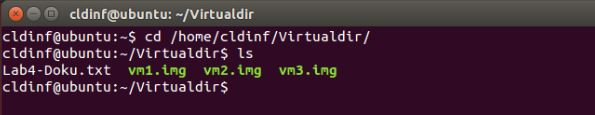
\includegraphics[width=0.80\textwidth]{./pictures/virtualdir.jpg}
	\caption{{Virtualdir Übersicht}}
	\label{virtualdir}
	\end{center}
\end{figure}

\subsection{Networking}
In diesem Kapitel werden einige Konfigurationsdetails zum Netzwerk aufgezeigt. 

\subsubsection{Host-Networkconfig}
Host IP Konfiguration und Tabs 

\subsubsection{Guest-Networkconfig}
Netzwerkkonfig von den Guests 

\subsubsection{Bridge}
Hier folgen die Daten der Bridge

\section{Anleitung}
Es wird von Ubuntu 14.04 als Hosts-OS ausgegangen.
Was wird benötigt:
\begin{itemize}

\item Ein Guest-OS Image
\end{itemize}

\subsubsection{Vorbereitung}
\begin{itemize}
\item Installation der Virtualisierungssoftware \textbf{QEMU}:
\begin{lstlisting}
sudo apt-get install qemu-system-x86_64
sudo apt-get install qemu-utils
\end{lstlisting}
\item Installation des Packets \textbf{bridge-utils} für das Bridgemanagement:
\begin{lstlisting}
sudo apt-get install bridge-utils
\end{lstlisting}
\end{itemize} 

\begin{itemize}
\item Erweitere Zugriffsrechte auf das \textbf{TUN-Device} für group und others:
\begin{lstlisting}
sudo chmod go+rw /dev/net/tun
\end{lstlisting}
\end{itemize}

\begin{itemize}
\item Anpassen der \textbf{QEMU} Interface up \& down Skripte:
\newline
Jeweils die Inhalte ersetzen:
\newline
/etc/qemu-ifup:
\begin{lstlisting}
#!/bin/sh                                                        
sudo /sbin/ifconfig $1 0.0.0.0 up
\end{lstlisting}
/etc/qemu-ifdown:
\begin{lstlisting}
#!/bin/sh                                                        
sudo /sbin/ifconfig $1 0.0.0.0 up
\end{lstlisting}
\end{itemize}

\begin{itemize}
\item Sofern \textbf{qemu-ifup} \& \textbf{qemu-ifdown} nicht bereits ausführbar sind, dies nachholen:
\begin{lstlisting}
sudo chmod +x /etc/qemu-ifup
sudo chmod +x /etc/qemu-ifdown
\end{lstlisting}
\end{itemize}
\subsubsection{Guest-OS}
\begin{itemize}
\item Starten der VM's mittels QEMU und erzeugen der \textbf{TAP}'s:
\begin{lstlisting}
sudo qemu-system-x86_64 vm.img -net nic, -net tap,ifname=tapext -net nic, -net tap,ifname=tap12
sudo qemu-system-x86_64 vm.img -net nic, -net tap,ifname=tap21 -net nic, -net tap,ifname=tap23
sudo qemu-system-x86_64 vm.img -net nic, -net tap,ifname=tap32
\end{lstlisting}
Die TAP's und Bridges sollten nun bei der Eingabe von \textit{ifconfig} ersichtlich sein.

\item In den Guest-OS müssen den Netzwerkinterfaces IP-Adressen zugewiesen werden. Die folgenden Befehlesind in den Guest-OS auszuführen.
\newline
VM1:
\begin{lstlisting}
ifconfig eth0 10.10.0.2 netmask 255.255.255.0 up
ifconfig eth1 10.10.1.2 netmask 255.255.255.0 up
\end{lstlisting}
VM2:
\begin{lstlisting}
ifconfig eth0 10.10.1.3 netmask 255.255.255.0 up
ifconfig eth1 10.10.2.2 netmask 255.255.255.0 up
\end{lstlisting}
VM3:
\begin{lstlisting}
ifconfig eth1 10.10.2.2 netmask 255.255.255.0 up

\end{lstlisting}


\end{itemize}

\subsubsection{Bridges}
\begin{itemize}
\item Erstellen der \textbf{Bridges}:
\begin{lstlisting}
brctl addbr brext
brctl addbr br121
brctl addbr br323
\end{lstlisting}



\item Die durch das starten der VM's erstellten TAPS müssen nun den Bridges zugeordnet werden.
\newline
Bridge \textbf{brext}:
\begin{lstlisting}
sudo brctl addif brext eth0
sudo brctl addif brext tapext
\end{lstlisting}
Bridge \textbf{br121}:
\begin{lstlisting}
sudo brctl addif br121 tap12
sudo brctl addif br121 tap21
\end{lstlisting}
Bridge \textbf{br323}:
\begin{lstlisting}
sudo brctl addif br323 tap23
sudo brctl addif br323 tap32
\end{lstlisting}


\item Den Bridges die \textbf{IP's zuweisen}:
\begin{lstlisting}
sudo ifconfig brext 10.10.0.1 netmask 255.255.255.0 up
sudo ifconfig br121 10.10.1.1 netmask 255.255.255.0 up
sudo ifconfig br323 10.10.2.1 netmask 255.255.255.0 up
\end{lstlisting}






\end{itemize}
\end{document}
